\documentclass[review, 12pt]{elsarticle}

\usepackage{hyperref}
\usepackage{lineno}
\modulolinenumbers[1]

\journal{BJU International}
%\usepackage{fancyhdr}
%\rhead{\thepage}
\usepackage{fancyhdr}
\pagestyle{fancy}
\fancyhf{}
\renewcommand{\headrulewidth}{0pt}
\fancyhead[R]{\thepage}

%\usepackage{fig2vect}
\usepackage{graphicx}
%\usepackage{svg}
\usepackage{booktabs}
%\usepackage[swedish, english]{babel}

%%%%%%%%%%%%%%%%%%%%%%%
%% Elsevier bibliography styles
%%%%%%%%%%%%%%%%%%%%%%%
%% To change the style, put a % in front of the second line of the current style and
%% remove the % from the second line of the style you would like to use.
%%%%%%%%%%%%%%%%%%%%%%%

%% Numbered
%\bibliographystyle{model1-num-names}

%% Numbered without titles
%\bibliographystyle{model1a-num-names}

%% Harvard
%\bibliographystyle{model2-names.bst}\biboptions{authoryear}

%% Vancouver numbered
\usepackage{numcompress}\bibliographystyle{model3-num-names}

%% Vancouver name/year
%\usepackage{numcompress}\bibliographystyle{model4-names}\biboptions{authoryear}

%% APA style
%\bibliographystyle{model5-names}\biboptions{authoryear}

%% AMA style
%\usepackage{numcompress}\bibliographystyle{model6-num-names}

%% `Elsevier LaTeX' style
%\bibliographystyle{elsarticle-num}
%%%%%%%%%%%%%%%%%%%%%%%

%\renewcommand{\familydefault}{\sfdefault}

\begin{document}

\begin{frontmatter}

\title{Personalized Biopsy Schedules Based on Risk of Gleason Upgrading for Low-Risk Prostate Cancer Active Surveillance Patients\tnoteref{wordcount}}
\tnotetext[wordcount]{Word count: 3306}

%% Group authors per affiliation:
\author[1]{Anirudh Tomer\corref{corauthor}, MSc} 
\cortext[corauthor]{Corresponding author (Anirudh Tomer): Erasmus MC, kamer flex Na-2823, PO Box 2040, 3000 CA Rotterdam, the Netherlands. Tel: +31 10 70 43393.}
\ead{a.tomer@erasmusmc.nl}

\author[2,3]{Daan Nieboer, MSc}
\ead{d.nieboer@erasmusmc.nl}

\author[3]{Monique J. Roobol, PhD}
\ead{m.roobol@erasmusmc.nl}

\author[4]{Anders Bjartell, MD, PhD}
\ead{anders.bjartell@med.lu.se}

\author[2,5]{Ewout W. Steyerberg, PhD}
\ead{e.w.steyerberg@lumc.nl}

\author[1]{Dimitris Rizopoulos, PhD}
\ead{d.rizopoulos@erasmusmc.nl}

\author[6]{Movember Foundation's Global Action Plan Prostate Cancer Active Surveillance (GAP3) consortium}

\address[1]{Department of Biostatistics, Erasmus University Medical Center, Rotterdam, the Netherlands}
\address[2]{Department of Public Health, Erasmus University Medical Center, Rotterdam, the Netherlands}
\address[3]{Department of Urology, Erasmus University Medical Center, Rotterdam, the Netherlands}
\address[4]{Department of Urology, Sk\r{a}ne University Hospital, Malm\"{o}, Sweden}
\address[5]{Department of Biomedical Data Sciences, Leiden University Medical Center, Leiden, the Netherlands}
\address[6]{The Movember Foundation's Global Action Plan Prostate Cancer Active Surveillance (GAP3) consortium members presented in Appendix A}

%% or include affiliations in footnotes:

% !TEX root =  ../main_manuscript.tex 
\begin{abstract}
\texttt{Background}: Prostate cancer active surveillance (AS) patients undergo repeat biopsies. Active treatment is advised when biopsy Gleason grade group~$\geq$~2 (\textit{upgrading}). Many patients never experience upgrading, yet undergo biopsies frequently. Personalized biopsy decisions based on upgrading-risk may reduce patient burden.\\

\texttt{Objective}: Develop a risk prediction model and web-application to assist patients/doctors in personalized biopsy decisions.\\

\texttt{Design, Setting, and Participants}: Model development: world's largest AS study PRIAS, 7813 patients, 1134 experienced upgrading; External validation: largest five cohorts of Movember Foundation's GAP3 database (${>20,000}$ patients, 27 centers worldwide); Data: repeat prostate-specific antigen (PSA) and biopsy Gleason grade.\\

\texttt{Outcome Measurements, and Statistical Analysis}: A Bayesian joint model fitted to the PRIAS dataset. This model was validated in GAP3 cohorts using risk prediction error, calibration, area under ROC (AUC). Model and personalized biopsy schedules based on predicted risks were implemented in a web-application.\\

\texttt{Results and Limitations}: Cause-specific cumulative upgrading-risk at year five of follow-up: 35\% in PRIAS, at most 50\% in GAP3 cohorts. PRIAS based model: PSA velocity was a stronger predictor of upgrading (Hazard~Ratio:~2.47, 95\%CI:~1.93--2.99) than PSA value (Hazard~Ratio:~0.99, 95\%CI:~0.89--1.11). Validation: Moderate AUC (0.55--0.75) in PRIAS and GAP3 cohorts. Moderate prediction error (0.1--0.3) in GAP3 cohorts where impact of PSA value and velocity on upgrading-risk was similar to PRIAS, but large (0.3--0.45) otherwise. Recalibration advised for external cohorts.\\

\texttt{Conclusions}: We successfully developed and validated a model for predicting upgrading-risk, and providing risk-based personalized biopsy decisions, in prostate cancer AS. The model made available via a web-application enables shared decision making of biopsy schedules by comparing fixed and personalized schedules on total biopsies and expected time delay in detecting upgrading.\\

\texttt{Patient Summary}: Personalized prostate biopsies are a novel alternative to fixed one-size-fits-all schedules. The underlying statistical models are made available through a user-friendly web-application and may help to reduce unnecessary prostate biopsies while maintaining cancer control.
\end{abstract}
%Word count: 300 words excluding headings

\begin{keyword}
Active Surveillance\sep Biopsies \sep Personalized Medicine\sep Prostate Cancer \sep Shared Decision Making.
\end{keyword}

\end{frontmatter}

%Adding and removing line numbers
\linenumbers

% !TEX root =  ../main_manuscript.tex 
\section{Introduction}
Patients with low- and very low-risk screening-detected localized prostate cancer are usually advised active surveillance (AS) instead of immediate radical treatment~\citep{briganti2018active}. In AS, cancer progression is routinely monitored via prostate-specific antigen (PSA), digital rectal examination, and repeat biopsies. Among these, the strongest indicator of cancer-related outcomes is the biopsy Gleason grade~\citep{epsteinGG2014}. When the Gleason grade increases from grade~1 (Gleason 3+3) to 2 (Gleason 3+4) or higher, called \textit{reclassification}, patients are commonly advised curative treatment~\citep{bul2013active}.

\begin{figure}
\centerline{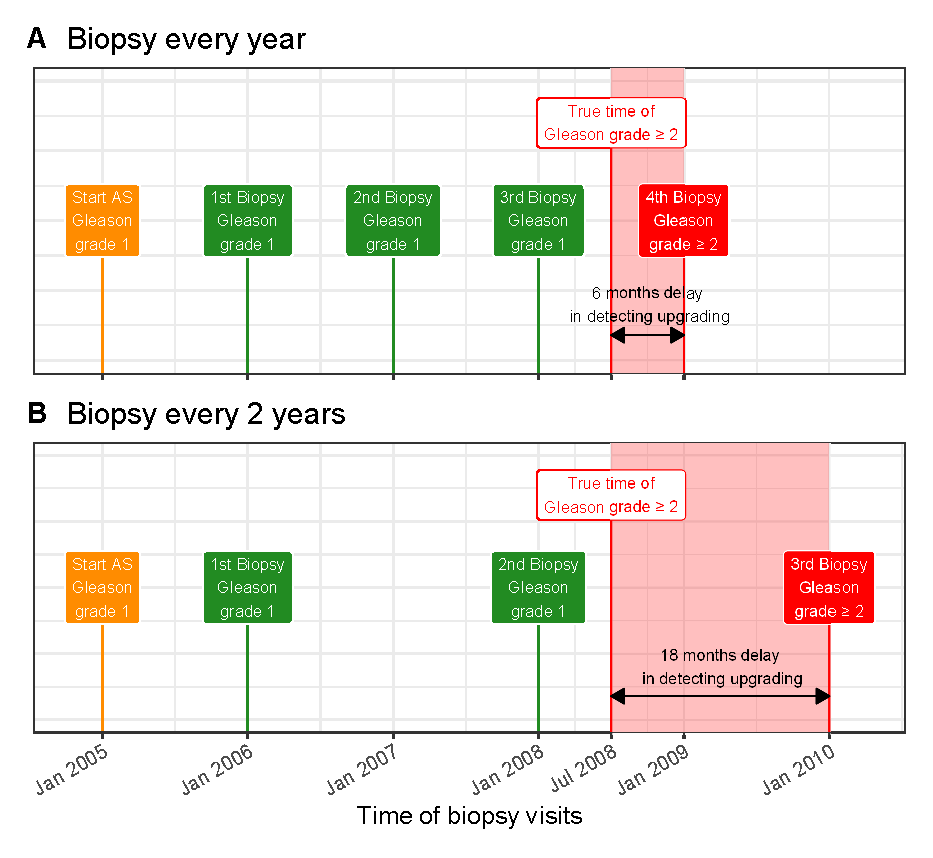
\includegraphics[width=\columnwidth]{images/delay_explanation.eps}}
\caption{\textbf{Trade-off between the number of biopsies and time delay in detecting reclassification (Increase in Gleason grade from 1 to 2 or higher):} The true time of reclassification for the patient in this figure is July 2008. When biopsies are scheduled annually (\textbf{Panel~A}), reclassification is detected in January 2009 with a time delay of six months, and a total of four biopsies are scheduled. When biopsies are scheduled biennially (\textbf{Panel~B}) reclassification is detected in January 2010 with a time delay of 18 months, and a total of three biopsies are scheduled. Since biopsies are conducted periodically, the time of reclassification is observed as an interval. For example, between Jan~2008--Jan~2009 in \textbf{Panel~A} and between Jan~2008--Jan~2010 in \textbf{Panel~B}.}
\label{fig:delay_explanation}
\end{figure}

Biopsies are conducted periodically. Consequently, reclassification is always detected with a time delay (Figure~\ref{fig:delay_explanation}). For detecting reclassification timely, many AS programs schedule fixed and frequent biopsies (e.g.,~annually) for all patients~\citep{nieboer2018active,loeb2014heterogeneity}. However, this also leads to many unnecessary biopsies in slow/non-progressing patients. Biopsies are invasive, painful and prone to medical complications. Thus, biopsy burden and patient non-compliance to frequent biopsies~\citep{bokhorst2015compliance} has raised concerns regarding the optimal biopsy schedule~\citep{inoue2018comparative, bratt2013study}. To this end, infrequent schedules such as biennial biopsies have been proposed as an alternative~\citep{inoue2018comparative,de2017estimating}. Although, biennial biopsies may still lead to five unnecessary biopsies over ten years (current study period of large AS programs) for slow/non-progressing patients. A promising alternative to fixed and frequent biopsies is personalized biopsy schedules based on the patient-specific risk of reclassification (Figure~\ref{fig:riskBasedExample}).

\begin{figure}
\centerline{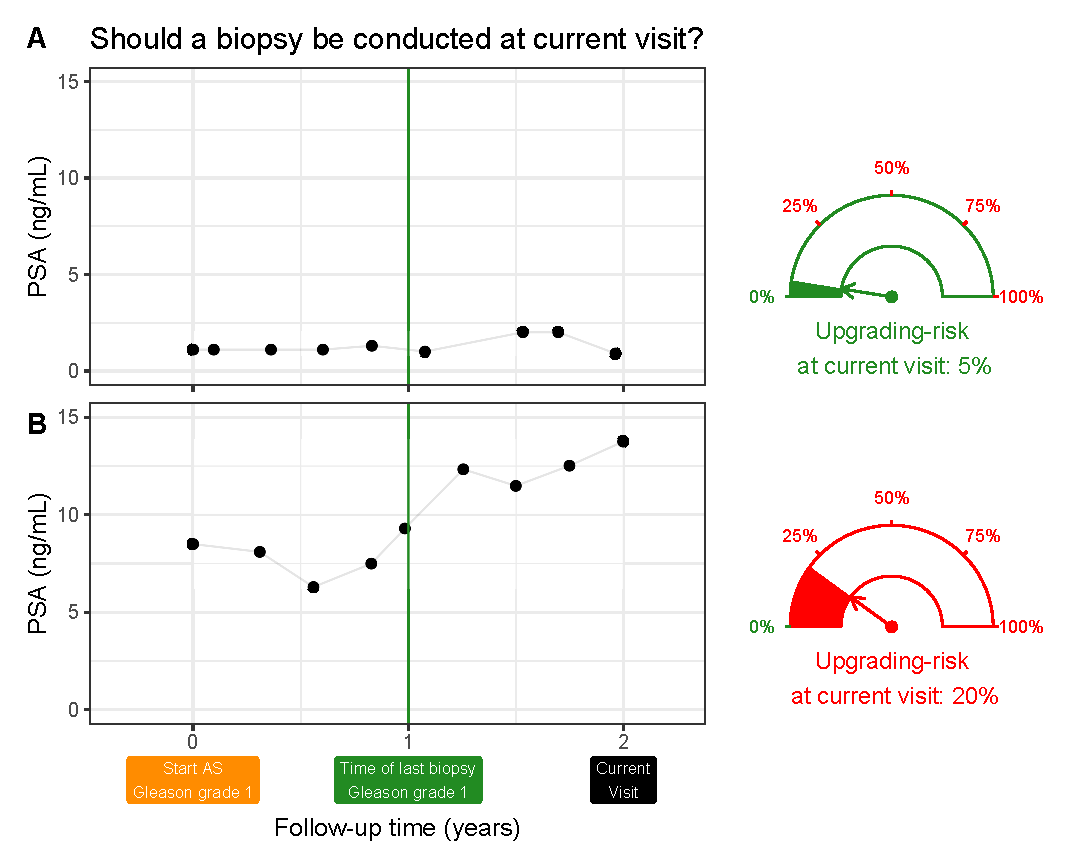
\includegraphics[width=\columnwidth]{images/riskBasedExample.eps}}
\caption{\textbf{Motivation for personalized risk-based decisions of biopsy}: Patient~A (\textbf{Panel~A}) and B (\textbf{Panel~B}) had their latest biopsy at year one of follow-up (green vertical line). Patient~A's prostate-specific antigen (PSA) profile remained stable until his current visit at year three, whereas patient~B's profile has shown a rise. Consequently, patient~B's estimated cumulative risk of reclassification at the current visit (year three) is higher than that of patient~A. This makes patient~B a more suitable candidate for biopsy than Patient~A. Risk estimates in this figure are only illustrative.}
\label{fig:riskBasedExample}
\end{figure}

The first challenge in developing personalized biopsy schedules is consolidating accumulated patient data (e.g., PSA, previous biopsy results) into risk estimates for reclassification. Existing calculators for risk of reclassification~\citep{partin1993use,makarov2007updated} use only the latest PSA measurement of a patient. In contrast, we intend to utilize all repeated measurements of PSA, previous biopsy results, and baseline characteristics of a patient. To this end, a suitable model is the joint model for time-to-event and longitudinal data~\citep{tomer2019, coley2017prediction,rizopoulos2012joint}. A joint model predicts risk of reclassification in a personalized manner. A subsequent challenge however, is translating risks into clinical decisions. For example, a 10\% risk of reclassification can be perceived high/low depending upon the patient age. Patients may also weigh risks of reclassification with the potential \textit{consequences} of another biopsy. Two relevant \textit{consequences} of biopsies (Figure~\ref{fig:delay_explanation}) are the timing and total number of biopsies (burden), and the time delay in detecting reclassification (smaller is beneficial). The relative importance of these \textit{consequences} can vary between the patients, and also over the follow-up period for the same patient.

The goal of this work was to assist patients and doctors in making better decisions of biopsies than fixed and frequent biopsies. For this purpose, we developed a web-application that gives patients their current and future risk of reclassification. It also suggests them risk-based personalized schedules of biopsies. For each biopsy schedule, be it fixed or personalized, the web-application provides expected \textit{consequences} of following it. Thus, patients can compare schedules before making a decision. The web-application uses a prediction joint model fitted to the world's largest AS dataset, PRIAS~\citep{bul2013active}. We externally validated this model in five largest AS cohorts of the GAP3 database \citep{gap3_2018}. Thus, the web-application can be used by a large number of patients worldwide.
%Intro: 605 words
%Cumsum: 605 words
% !TEX root =  ../main_manuscript.tex 
\section{Patients and Methods}
\subsection{Study Cohort}
\label{subsec:cohort}
For developing a statistical model to predict upgrading-risk, we used the world's largest AS dataset, Prostate Cancer International Active Surveillance or PRIAS~\citep{bul2013active}, dated April 2019 (Table~\ref{table:prias_summary}). In PRIAS, biopsies were scheduled at year one, four, seven, ten, and additional yearly biopsies were scheduled when PSA doubling time was between zero and ten years. We selected all 7813~patients who had Gleason grade group~1 at inclusion in AS. Our primary event of interest is an increase in this Gleason grade group observed upon repeat biopsy, called \textit{upgrading} (1134~patients). Upgrading is a trigger for treatment advice in PRIAS. Also, 2250~patients were provided treatment based on their PSA, the number of biopsy cores with cancer, or anxiety/other reasons. However, our reasons for focusing solely on upgrading are that upgrading is strongly associated with cancer-related outcomes, and other treatment triggers vary between cohorts~\citep{nieboer2018active}.

For externally validating our model's predictions, we selected the following largest (by the number of repeated measurements) six cohorts from Movember Foundation's GAP3 database~\citep{gap3_2018} version~3.1, covering nearly 73\% of the GAP3 patients: the University of Toronto AS (Toronto), Johns Hopkins AS (Hopkins), Memorial Sloan Kettering Cancer Center AS (MSKCC), King's College London AS (KCL), Michigan Urological Surgery Improvement Collaborative AS (MUSIC), and University of California San Francisco AS (UCSF, version~3.2). Only patients with a Gleason grade group~1 at the time of inclusion in these cohorts were selected. Summary statistics are presented in Supplementary~A.2.

\begin{table}
\small\sf\centering
\caption{\textbf{Summary of the PRIAS dataset as of April 2019}. The primary event of interest is upgrading, that is, increase in Gleason grade group from group~1~\citep{epsteinGG2014} to 2 or higher. IQR:~interquartile range, PSA:~prostate-specific antigen. Study protocol URL: \url{https://www.prias-project.org}}
\label{table:prias_summary}
\begin{tabular}{lr}
\toprule
\textbf{Characteristic} & \textbf{Value}\\
\midrule
%Total centers & $> 100$\\
Total patients & 7813\\
Upgrading (primary event) & 1134\\
Treatment & 2250\\
Watchful waiting & 334\\
Loss to follow-up & 249\\
Death (unrelated to prostate cancer) & 95\\
Death (related to prostate cancer) & 2\\
\midrule
Median age at diagnosis (years) & 66 (IQR: 61--71)\\
Median maximum follow-up per patient (years) &  1.8 (IQR: 0.9--4.0)\\
Total PSA measurements & 67578\\
Median number of PSA measurements per patient &  6 (IQR: 4--12)\\
Median PSA value (ng/mL) & 5.7 (IQR: 4.1--7.7)\\
Total biopsies & 15686\\
Median number of biopsies per patient &  2 (IQR: 1--2)\\
\bottomrule
\end{tabular}
\end{table}

\paragraph{Choice of predictors:} In our model, we used all repeated PSA measurements, the timing of the previous biopsy and Gleason grade, and age at inclusion in AS. Other predictors such as prostate volume, MRI results can also be important. MRI is utilized already for targeting biopsies, but regarding its use in deciding the time of biopsies, there are arguments both for and against it~\citep{kasivisvanathan2020magnetic,chesnut2019role,schoots2015magnetic}. MRI is still a recent addition in most AS protocols. Consequently, repeated MRI data is very sparsely available in both PRIAS and GAP3 databases to make a stable prediction model. Prostate volume data is also sparsely available, especially in validation cohorts. Based on these reasons, we did not include them in our model. However, the model we propose next is extendable to include MRI and other novel biomarkers in the future.
%Study cohort: 370 words
%Cumsum: 975 words
% !TEX root =  ../main_manuscript.tex 
\subsection{Statistical Model}
Modeling an AS dataset such as PRIAS, posed certain challenges. First, PSA was measured longitudinally, and over follow-up time it did not always increase linearly. Consequently, we expect that PSA measurements of a patient are more similar to each other than of another patient. In other words, we need to accommodate the within-patient correlation for PSA. Second, PSA was available only until a patient observed upgrading. Thus, we also need to model the association between the Gleason grades and PSA profiles of a patient, and handle missing PSA measurements after a patient experienced upgrading. Third, since the PRIAS biopsy schedule uses PSA, a patient's observed time of upgrading was also dependent on their PSA. Thus, the effect of PSA on the upgrading-risk need to be adjusted for the effect of PSA on the biopsy schedule. Fourth, many patients obtained treatment and watchful waiting before observing upgrading. Since we considered events other than upgrading as censoring, the model needs to account for patients' reasons for treatment or watchful waiting (e.g., age, treatment based on observed data). A model that handles these challenges in a statistically sound manner is the joint model for time-to-event and longitudinal data~\citep{tomer2019,coley2017prediction,rizopoulos2012joint}.

Our joint model consisted of two sub-models. Namely, a linear mixed-effects sub-model~\citep{laird1982random} for longitudinally measured PSA (log-transformed), and a relative-risk sub-model (similar to the Cox model) for the interval-censored time of upgrading. Patient age was used in both sub-models. Results and timing of the previous negative biopsies were used only in the risk sub-model. To account for PSA fluctuations~\citep{nixon1997biological}, we assumed t-distributed PSA measurement errors. The correlation between PSA measurements of the same patient was established using patient-specific random-effects. We fitted a unique curve to the PSA measurements of each patient (Panel~A, Figure~\ref{fig:jmExplanationPlot_113}). Subsequently, we calculated the mathematical derivative of the patient's fitted PSA profile (Equation~2, Supplementary~A), to obtain his follow-up time specific instantaneous PSA velocity (Panel~B, Figure~\ref{fig:jmExplanationPlot_113}). This instantaneous velocity is a stronger predictor of upgrading than the widely used average PSA velocity~\citep{cooperberg2018refined}. We modeled the impact of PSA on upgrading-risk by employing fitted PSA value and instantaneous velocity as predictors in the risk sub-model (Panel~C, Figure~\ref{fig:jmExplanationPlot_113}). We adjusted the effect of PSA on upgrading-risk for the PSA dependent PRIAS biopsy schedule by estimating parameters using a full likelihood method (proof in Supplementary~A). This approach also accommodates watchful waiting and treatment protocols that are also based on patient data. Specifically, the parameters of our two sub-models were estimated jointly under the Bayesian paradigm (Supplementary~A) using the R package \textbf{JMbayes}~\citep{rizopoulosJMbayes}.

\begin{figure}
\centerline{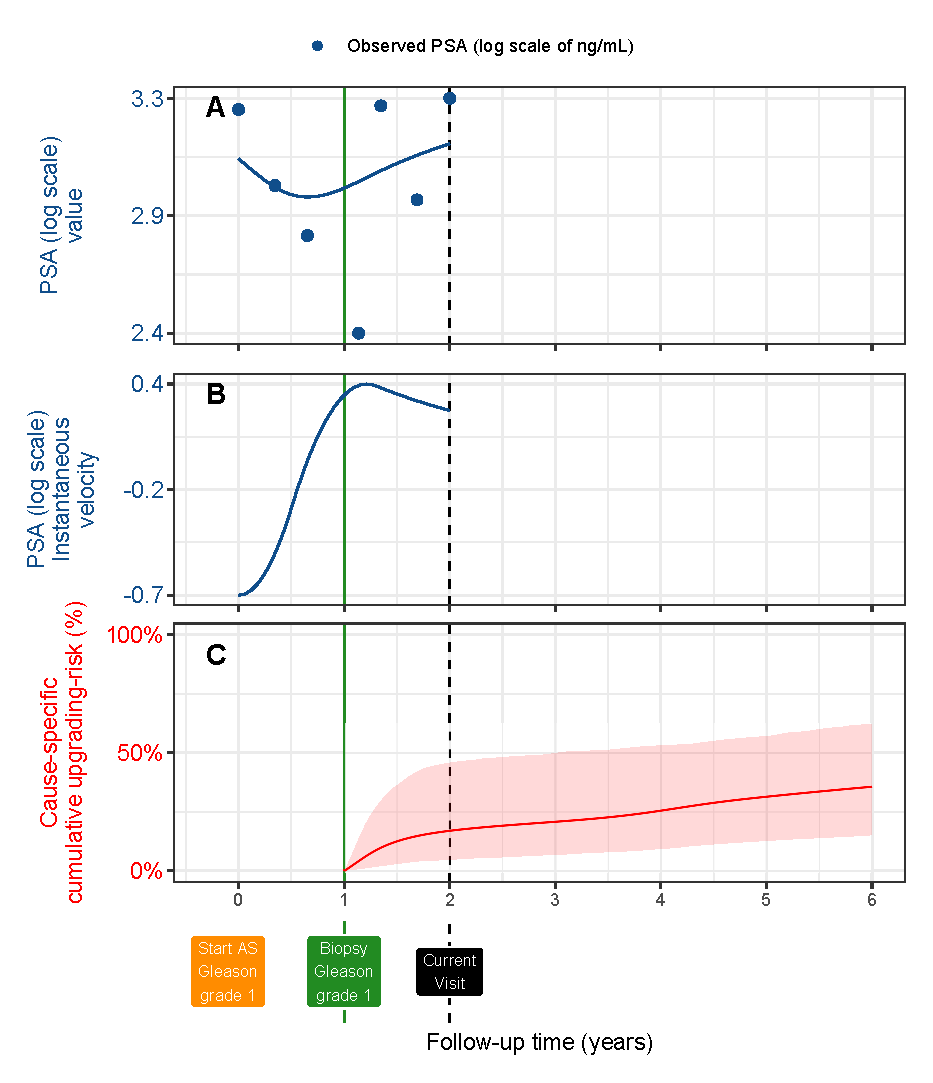
\includegraphics[width=\columnwidth]{images/jmExplanationPlot_113.eps}}
\caption{\textbf{Illustration of the joint model on a real PRIAS patient}. \textbf{Panel~A:} Observed PSA (blue dots) and fitted PSA (solid blue line), log-transformed from ng/mL. \textbf{Panel~B:} Estimated instantaneous velocity of PSA (log-transformed). \textbf{Panel~C}: Predicted cause-specific cumulative upgrading-risk (95\% credible interval shaded). Upgrading is defined as an increase in the Gleason grade group from group~1~\citep{epsteinGG2014} to 2 or higher. This upgrading-risk is calculated starting from the time of the latest negative biopsy (vertical green line at year one of follow-up). The joint model estimated it by combining the fitted PSA (log scale) value and instantaneous velocity, and time of the latest negative biopsy. Black dashed line at year two denotes the time of current visit.}
\label{fig:jmExplanationPlot_113}
\end{figure}

\subsection{Risk Prediction and Model Validation}
Our model provides predictions for upgrading-risk over the entire future follow-up period of a patient (Panel~C, Figure~\ref{fig:jmExplanationPlot_113}). However, we recommend using predictions only after year one. This is because most AS programs recommend a confirmatory biopsy at year one, especially to detect patients who may be misdiagnosed as low-grade at inclusion in AS. The risk predictions for a patient are not calculated only once. Rather, as illustrated in Figure~5 of Supplementary~B, risk-predictions update over the follow-up, to account for additional patient data (e.g., new biopsy results, PSA measurements) that becomes available. We validated our model internally in the PRIAS cohort, and externally in the largest six GAP3 database cohorts. We employed calibration plots~\citep{royston2013external,steyerberg2010assessing} and follow-up \textit{time-dependent} mean absolute risk prediction error or MAPE~\citep{rizopoulos2017dynamic} to graphically and quantitatively evaluate our model's risk prediction accuracy, respectively. We assessed our model's ability to discriminate between patients who experience/do not experience upgrading via the time-dependent area under the receiver operating characteristic curve or AUC~\citep{rizopoulos2017dynamic}. 

The aforementioned \textit{time-dependent} AUC and MAPE~\citep{rizopoulos2017dynamic} are temporal extensions of their standard versions~\citep{steyerberg2010assessing} in a longitudinal setting. Specifically, at every six months of follow-up, we calculated a unique AUC and MAPE for predicting upgrading-risk in the subsequent one year (Supplementary~B.1). For emulating a realistic situation, we calculated the AUC and MAPE at each follow-up using only the validation data available until that follow-up. For example, calculations for AUC and MAPE for the time interval year two to year three do not utilize data of patients who progressed before year two. Last, to resolve any potential model miscalibration in validation cohorts, we aimed to recalibrate our model's baseline hazard of upgrading (Supplementary~B.1), individually for each cohort.
%Stat analysis: 621 words
%Cumsum: 1596 words
% !TEX root =  ../main_manuscript.tex 
\section{Results}
\subsection{General Results}
In PRIAS, the probability of experiencing reclassification within the first five and ten years was 33\% and 42\%, respectively (cumulative-risk plot in Appendix A). That is, ideally more than 50\% of the patients may not require any biopsy in the first ten years.

\subsection{Joint Model Results} 
For every ten years increase in a patient age at the time diagnosis, the adjusted hazard ratio of reclassification is 1.45~(95\%CI:~1.30--1.63). When fitted PSA value (log scale) increases from 2.36 (25-th percentile of fitted PSA) to 3.07 (75-th percentile of fitted PSA), the adjusted hazard ratio of reclassification is 0.99~(95\%CI:~0.89--1.11). When estimated instantaneous PSA (log scale) velocity increases from -0.09 (25-th percentile of estimated velocity) to 0.31 (75-th percentile of estimated velocity), the adjusted hazard ratio of reclassification is 2.47~(95\%CI:~1.93--2.99). Hence, the instantaneous PSA (log scale) velocity is a stronger predictor for hazard of reclassification than the PSA value (log scale). Detailed parameter estimates are in Appendix~A.4.

\subsection{Validation Results}
Using the joint model fitted to the PRIAS dataset we made risk predictions for GS7 in real PRIAS patients. As shown in Figure 4 of Appendix B, these risk estimates become more accurate as more data is gathered over follow-up. To check the accuracy of these risk predictions, we calculated the time dependent area under the receiver operating characteristic curves (AUC) as a measure of discrimination, and the root mean squared prediction error (RMSPE) as a measure of calibration. These are shown in Figure~\ref{fig:auc_pe}. For predictions within PRIAS (internal validation), the time-dependent AUC was between 0.62 and 0.69, and RMSPE between 0.23 and 0.37 over the whole follow-up period. For validation in external cohorts, the AUC was similar to the AUC of PRIAS for all cohorts during the first three years of follow-up. The RMPSE however differed much more during the same period. The AS cohorts closest to PRIAS in terms of RMSPE were Johns Hopkins Active Surveillance and Memorial Sloan Kettering Cancer Center Active Surveillance. Detailed AUC and RMSPE results for all cohorts with 95\% bootstrapped confidence intervals are presented in Table 6 to Table 11 of Appendix B.

\begin{figure}
\centerline{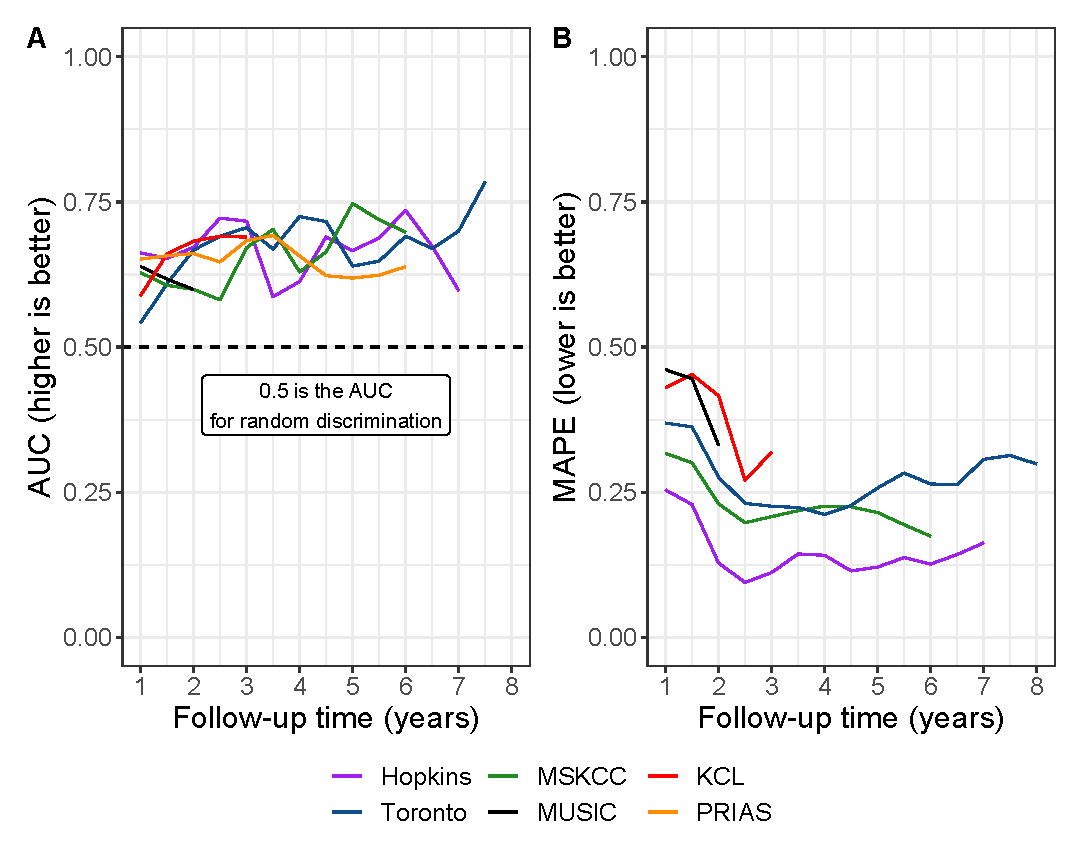
\includegraphics[width=\columnwidth]{images/auc_pe.eps}}
\caption{\textbf{Validation of predictions of Gleason $\geq$ 7 (GS7)}. In \textbf{Panel~A} we can see that the time dependent area under the receiver operating characteristic curve or AUC (measure of discrimination) is above 0.5 in PRIAS (internal validation), and in Toronto, JHAS, MSKCC, KCL, and MUSIC AS cohorts (external validation). In \textbf{Panel~B} we can see that the time dependent root mean squared prediction error or RMSPE (measure of calibration) is similar for PRIAS, and JHAS and Toronto cohorts. The bootstrapped 95\% confidence interval for these estimates are presented in Table 6 to Table 11 of Appendix B. Full names of Cohorts are \textit{PRIAS}: Prostate Cancer International Active Surveillance, \textit{Toronto}: University of Toronto Active Surveillance, \textit{JHAS}: Johns Hopkins Active Surveillance, \textit{MSKCC}: Memorial Sloan Kettering Cancer Center Active Surveillance, \textit{KCL}: King's College London Active Surveillance, \textit{MUSIC}: Michigan Urological Surgery Improvement Collaborative Active Surveillance.}
\label{fig:auc_pe}
\end{figure}

\subsection{Personalized Schedule Results}
Using the risk predictions for GS7, we developed personalized schedules of biopsy for real PRIAS patients. We maintained a minimum gap of one year between biopsies as advised by the PRIAS protocol. In addition, we scheduled biopsies only for the first ten years follow-up because of limited follow-up period of the training dataset PRIAS. A compulsory biopsy was done scheduled year ten of follow-up in all schedules for meaningful comparison of their expected delays in detection of GS7. Various personalized and fixed biopsy schedules for demo patients are shown in Figure \ref{fig:demo_pat1} and Appendix C's Figure 6, 7, 8 and 9. The biopsies denoted by `B' show that personalized schedules schedule fewer biopsies than fixed schedules. At the same time the expected time delay in detection of GS7 is less than an year for personalized schedules. We have implemented this approach in a web-application (\url{https://emcbiostatistics.shinyapps.io/prias_biopsy_recommender/}, and Appendix D) for practical use.
%Stat analysis: 650 words
%Cumsum: 2246 words
% !TEX root =  ../main_manuscript.tex 
\section{Discussion}
\label{sec:discussion}
In this paper, we presented a methodology to create personalized schedules for burdensome diagnostic \textit{tests} utilized to detect disease \textit{progression} in early-stage chronic non-communicable disease \textit{surveillance}. For this purpose, we utilized joint models for time-to-event and longitudinal data. Our approach first combines a patient's clinical data (e.g., longitudinal biomarkers) and previous invasive test results to estimate patient-specific cumulative-risk of disease progression over their current and future follow-up visits. We then plan future invasive tests whenever this cumulative-risk of progression is predicted to be above a certain threshold. We select the risk threshold automatically in a personalized manner, by optimizing a utility function of the patient-specific consequences of choosing a particular risk threshold based schedule. These consequences are, namely, the number of invasive tests (burden) planned in a schedule, and the expected time delay in detection of progression (shorter is beneficial) if the patient progresses. Last, we calculate this expected time delay in a personalized manner for both personalized and fixed schedules to assist patients/doctors in making a more informed decision of choosing a test schedule.

Using joint models gives us certain advantages. First, since joint models employ random-effects, the corresponding risk-based schedules are inherently personalized. Second, to predict this patient-specific risk of progression, joint models utilize all observed longitudinal measurements of a patient. Also, the continuous longitudinal outcomes are not discretized, which is commonly a case in Markov Decision Process and flowchart-based test schedules. Third, personalized schedules update automatically with more patient data over follow-up. Fourth, we calculated the expected number of tests (burden) and expected time delay in detecting progression (shorter is beneficial) in a patient-specific manner. Using our methodology, these can be calculated for both personalized and fixed schedules. Thus, patients/doctors can compare risk-based and fixed schedules and choose one according to their preferences for the expected burden-benefit ratio. Last, although this work concerns invasive test schedules in disease surveillance, the methodology is generic for use under a screening setting as well.

Personalized schedules that we proposed require a risk threshold. We optimized the threshold choice using a generic utility function based on the expected number of biopsies and time delay in detecting progression. We used only these two measures because they are easy to interpret but simultaneously critical for deciding the timing of invasive tests. Also, the time delay in detecting progression should manifest the window of opportunity for curative treatment and additional benefits of observing progression early. Practitioners may extend/modify this utility function by adding to/replacing time delay with commonly used decision-theoretic measures such as quality-adjusted life-years/expectancy (QALY/QALE).

We evaluated personalized schedules in a full cohort via a realistic simulation of a randomized clinical trial for prostate cancer surveillance patients. We observed that personalized schedules reduced many unnecessary biopsies for non-progressing patients compared to the widely used annual schedule. This happened at the cost of simultaneously having a slightly more time delay in detecting progression. Although, this delay should still be safe because it was almost equal to the delay of the world's largest prostate cancer active surveillance program PRIAS's schedule. The simulation study results are by no means the performance-limit of the personalized schedules. Instead, models with higher predictive accuracy and discrimination capacity than the PRIAS based model may lead to an even better balance between the number of tests and the time delay in detecting progression.

There are certain limitations to this work. First, in practice, most cohorts have a limited study period. Hence, the cumulative-risk profiles of patients and resulting personalized schedules can only be created up to the maximum study period. For this problem, the risk prediction model should be updated with more follow-up data over time. The proposed joint model assumed all events other than progression to be non-informative censoring. Alternative models that account for competing risks may lead to better results as they estimate absolute and not the cause-specific risk of progression. Upgrading is susceptible to inter-observer variation and sampling error. Although models that account for these two issues~\citep{balasubramanian2003estimation,coley2017prediction} will provide better risk estimates, the methodology for obtained personalized schedules can remain the same.
%Stat analysis: 759 words
%Cumsum: 3005 words
% !TEX root =  ../main_manuscript.tex 
\section{Conclusions}
We developed a novel methodology and model for personalized scheduling of biopsies in prostate cancer active surveillance (AS) patients. Unlike fixed biopsy schedules, personalized schedules utilize a patient's risk of reclassification to decide biopsies. They also update as more patient data becomes available over follow-up. Our model is externally validated in largest five AS cohorts of the GAP3 database. Our methodology is implemented in a web-application (\url{https://emcbiostatistics.shinyapps.io/prias_biopsy_recommender/}) and is accessible to large number of AS patients from the validated cohorts. To assist patients/doctors in making a share decision of an appropriate biopsy schedule, the web-application provides expected time delay in detection of reclassification (smaller is beneficial), and timing and total number of biopsies (burden), for both personalized and currently used fixed schedules.
%Conclusion: 104 words
%Cumsum: 3109 words

\section*{Author Contributions}
Anirudh Tomer had full access to all the data in the study and takes responsibility for the integrity of the data and the accuracy of the data analysis.

\noindent\textit{Study concept and design:} Tomer, Nieboer, Roobol, Bjartell, and Rizopoulos\\
\textit{Acquisition of data:} Tomer, Nieboer, and Roobol\\
\textit{Analysis and interpretation of data:} Tomer, Nieboer, and Rizopoulos\\
\textit{Drafting of the manuscript:} Tomer, and Rizopoulos\\
\textit{Critical revision of the manuscript for important intellectual content}: Tomer, Nieboer, Roobol, Bjartell, Steyerberg, and Rizopoulos\\
\textit{Statistical analyses}: Tomer, Nieboer, Steyerberg, and Rizopoulos\\
\textit{Obtaining funding}: Roobol, Steyerberg, and Rizopoulos\\
\textit{Administrative, technical or material support}: Nieboer\\
\textit{Supervision:} Roobol, and Rizopoulos\\
\textit{Other:} none
\section*{Acknowledgments}
The first and last authors would like to acknowledge support by Nederlandse Organisatie voor Wetenschappelijk Onderzoek (the national research council of the Netherlands) VIDI grant nr. 016.146.301, and Erasmus University Medical Center funding. Part of this work was carried out on the Dutch national e-infrastructure with the support of SURF Cooperative. The authors also thank the Erasmus University Medical Center's Cancer Computational Biology Center for giving access to their IT-infrastructure and software that was used for the computations and data analysis in this study.

This work was supported by the Movember Foundation. The funder did not play any role in the study design, collection, analysis or interpretation of data, or in the drafting of this paper.
\section*{Appendix A. Members of The Movember Foundation’s Global Action Plan Prostate Cancer Active Surveillance (GAP3) consortium}
\textit{Principle Investigators:} Bruce Trock (Johns Hopkins University, The James Buchanan Brady Urological Institute, Baltimore, USA), Behfar Ehdaie (Memorial Sloan Kettering Cancer Center, New York, USA), Peter Carroll (University of California San Francisco, San Francisco, USA), Christopher Filson (Emory University School of Medicine, Winship Cancer Institute,  Atlanta, USA), Jeri Kim / Christopher Logothetis (MD Anderson Cancer Centre, Houston, USA), Todd Morgan (University of Michigan and Michigan Urological Surgery Improvement Collaborative (MUSIC), Michigan, USA), Laurence Klotz (University of Toronto, Sunnybrook Health Sciences Centre, Toronto, Ontario, Canada),  Tom Pickles (University of British Columbia, BC Cancer Agency, Vancouver, Canada), Eric Hyndman (University of Calgary, Southern Alberta Institute of Urology, Calgary, Canada), Caroline Moore (University College London \& University College London Hospital Trust, London, UK), Vincent Gnanapragasam (University of Cambridge \& Cambridge University Hospitals NHS Foundation Trust, Cambridge, UK), Mieke Van Hemelrijck (King's College London, London, UK \& Guy’s and St Thomas’ NHS Foundation Trust, London, UK), Prokar Dasgupta (Guy’s and St Thomas’ NHS Foundation Trust, London, UK), Chris Bangma (Erasmus Medical Center, Rotterdam, The Netherlands/ representative of Prostate cancer Research International Active Surveillance (PRIAS) consortium), Monique Roobol (Erasmus Medical Center, Rotterdam, The Netherlands/ representative of Prostate cancer Research International Active Surveillance (PRIAS) consortium), Arnauld Villers (Lille University Hospital Center, Lille, France), Antti Rannikko (Helsinki University and Helsinki University Hospital, Helsinki, Finland), Riccardo Valdagni (Department of Oncology and Hemato-oncology, Università degli Studi di Milano, Radiation Oncology 1 and Prostate Cancer Program, Fondazione IRCCS Istituto Nazionale dei Tumori, Milan, Italy), Antoinette Perry (University College Dublin, Dublin, Ireland), Jonas Hugosson (Sahlgrenska University Hospital, Göteborg, Sweden), Jose Rubio-Briones (Instituto Valenciano de Oncología, Valencia, Spain), Anders Bjartell (Skåne University Hospital, Malmö, Sweden), Lukas Hefermehl (Kantonsspital Baden, Baden, Switzerland), Lee Lui Shiong (Singapore General Hospital, Singapore, Singapore), Mark Frydenberg (Monash Health; Monash University,  Melbourne, Australia), Yoshiyuki Kakehi / Mikio Sugimoto (Kagawa University Faculty of Medicine, Kagawa, Japan), Byung Ha Chung (Gangnam Severance Hospital, Yonsei University Health System, Seoul, Republic of Korea)

\textit{Pathologist:} Theo van der Kwast (Princess Margaret Cancer Centre, Toronto, Canada). 
Technology Research Partners: Henk Obbink (Royal Philips, Eindhoven, the Netherlands), Wim van der Linden (Royal Philips, Eindhoven, the Netherlands), Tim Hulsen (Royal Philips, Eindhoven, the Netherlands), Cees de Jonge (Royal Philips, Eindhoven, the Netherlands).

\textit{Advisory Regional statisticians:} Mike Kattan (Cleveland Clinic, Cleveland, Ohio, USA), Ji Xinge (Cleveland Clinic, Cleveland, Ohio, USA), Kenneth Muir (University of Manchester, Manchester, UK), Artitaya Lophatananon (University of Manchester, Manchester, UK), Michael Fahey (Epworth HealthCare, Melbourne, Australia), Ewout Steyerberg (Erasmus Medical Center, Rotterdam, The Netherlands), Daan Nieboer (Erasmus Medical Center, Rotterdam, The Netherlands); Liying Zhang (University of Toronto, Sunnybrook Health Sciences Centre, Toronto, Ontario, Canada)

\textit{Executive Regional statisticians:} Ewout Steyerberg (Erasmus Medical Center, Rotterdam, The Netherlands), Daan Nieboer (Erasmus Medical Center, Rotterdam, The Netherlands); Kerri Beckmann (King's College London, London, UK \& Guy’s and St Thomas’ NHS Foundation Trust, London, UK), Brian Denton (University of Michigan, Michigan, USA), Andrew Hayen (University of Technology Sydney, Australia), Paul Boutros (Ontario Institute of Cancer Research, Toronto, Ontario, Canada).

\textit{Clinical Research Partners’ IT Experts:} Wei Guo (Johns Hopkins University, The James Buchanan Brady Urological Institute, Baltimore, USA), Nicole Benfante (Memorial Sloan Kettering Cancer Center, New York, USA), Janet Cowan (University of California San Francisco, San Francisco, USA), Dattatraya Patil (Emory University School of Medicine, Winship Cancer Institute,  Atlanta, USA), Emily Tolosa (MD Anderson Cancer Centre, Houston, Texas, USA), Tae-Kyung Kim (University of Michigan and Michigan Urological Surgery Improvement Collaborative, Ann Arbor, Michigan, USA), Alexandre Mamedov (University of Toronto, Sunnybrook Health Sciences Centre, Toronto, Ontario, Canada), Vincent LaPointe (University of British Columbia, BC Cancer Agency, Vancouver, Canada), Trafford Crump (University of Calgary, Southern Alberta Institute of Urology, Calgary, Canada), Vasilis Stavrinides (University College London \& University College London Hospital Trust, London, UK), Jenna Kimberly-Duffell (University of Cambridge \& Cambridge University Hospitals NHS Foundation Trust, Cambridge, UK), Aida Santaolalla (King's College London, London, UK \& Guy’s and St Thomas’ NHS Foundation Trust, London, UK), Daan Nieboer (Erasmus Medical Center, Rotterdam, The Netherlands), Jonathan Olivier (Lille University Hospital Center, Lille, France), Tiziana Rancati (Fondazione IRCCS Istituto Nazionale dei Tumori di Milano, Milan, Italy), Helén Ahlgren (Sahlgrenska University Hospital, Göteborg, Sweden), Juanma Mascarós (Instituto Valenciano de Oncología, Valencia, Spain), Annica Löfgren (Skåne University Hospital, Malmö, Sweden), Kurt Lehmann (Kantonsspital Baden, Baden, Switzerland), Catherine Han Lin (Monash University and Epworth HealthCare, Melbourne, Australia), Hiromi Hirama (Kagawa University, Kagawa, Japan), Kwang Suk Lee (Yonsei University College of Medicine, Gangnam Severance Hospital, Seoul, Korea).  

\textit{Research Advisory Committee:} Guido Jenster (Erasmus MC, Rotterdam, the Netherlands), Anssi Auvinen (University of Tampere, Tampere, Finland), Anders Bjartell (Skåne University Hospital, Malmö, Sweden), Masoom Haider (University of Toronto, Toronto, Canada), Kees van Bochove (The Hyve B.V. Utrecht, Utrecht, the Netherlands), Ballentine Carter (Johns Hopkins University, Baltimore, USA – until 2018). 

\textit{Management team:} Sam Gledhill (Movember Foundation, Melbourne, Australia), Mark Buzza / Michelle Kouspou (Movember Foundation, Melbourne, Australia), Chris Bangma (Erasmus Medical Center, Rotterdam, The Netherlands), Monique Roobol (Erasmus Medical Center, Rotterdam, The Netherlands), Sophie Bruinsma / Jozien Helleman (Erasmus Medical Center, Rotterdam, The Netherlands).


\bibliography{bibliography}

\end{document}